


\section{Dataset construction at large scale}
\label{sec:Annot}

Our process of constructing large-scale object recognition image datasets consists of three key steps.

The first step is defining the set of target object categories.  To do this, we select from among the existing ImageNet~\citep{ImageNet} categories. By using WordNet as a backbone~\citep{WordNet}, ImageNet already takes care of disambiguating word meanings and of combining
together synonyms into the same object category. Since the selection of object categories needs to be done only
once per challenge task, we use a combination of automatic heuristics and manual post-processing to create the list of target
categories appropriate for each task. For example, for image classification we may include broader scene categories such as a type of beach,
but for single-object localization and object detection we want to focus only on object categories which can be unambiguously localized in images (Sections~\ref{sec:AnnotClsObjects} and~\ref{sec:AnnotDetObjects}).

The second step is collecting a diverse set of candidate images to represent the selected categories. We use both automatic and manual strategies on multiple search engines to do the image collection. The process is modified for the different ILSVRC tasks.
For example, for object detection we focus our efforts on collecting scene-like images using generic queries such as ``African safari'' to find pictures likely to contain multiple animals in one scene (Section~\ref{sec:AnnotDetImages}). 

The third (and most challenging) step is annotating the millions of collected images to obtain a clean dataset.
We carefully design crowdsourcing strategies targeted to each individual ILSVRC task. For example, the bounding box annotation system used for localization and detection tasks consists  of three distinct parts in order to include automatic crowdsourced quality control (Section~\ref{sec:AnnotLocBbox}).  Annotating images fully with all target object categories (on a reasonable budget) for object detection  requires an additional hierarchical image labeling system (Section~\ref{sec:AnnotDetList}).

We  describe the data collection and annotation procedure for each of the ILSVRC tasks in order: image classification (Section~\ref{sec:AnnotCls}), single-object localization (Section~\ref{sec:AnnotLoc}), and object detection (Section~\ref{sec:AnnotDet}), focusing on the three key steps for each dataset.

\begin{figure*}
\centering
%\includegraphics[width=6.75in]{diversity.png}
\begin{tabular}{r}
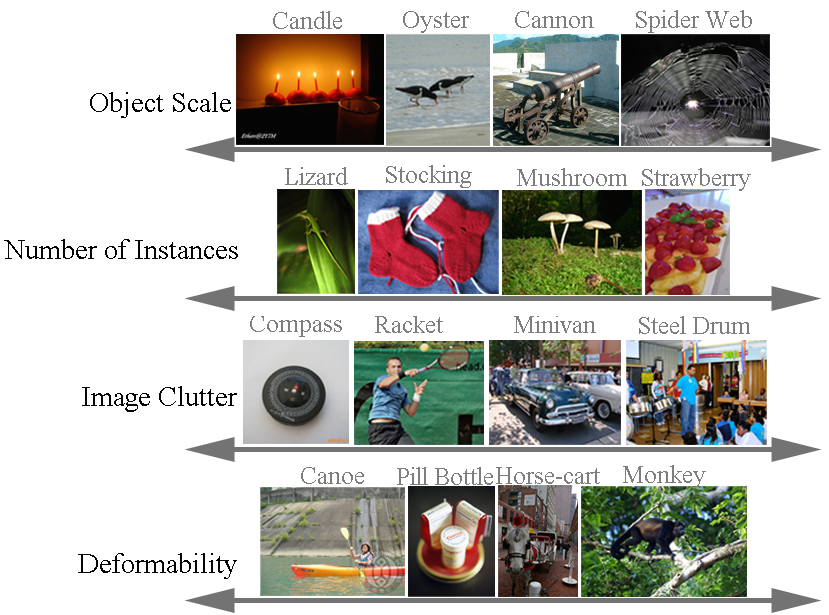
\includegraphics[width=5.5in]{diversity_left.png}\\
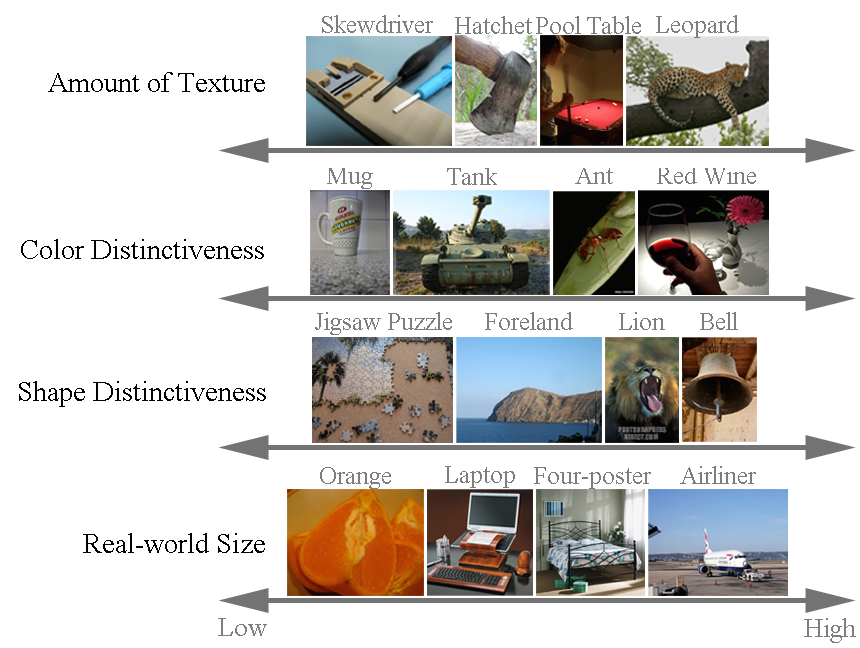
\includegraphics[width=5.7in]{diversity_right.png}
\end{tabular}
\caption{The diversity of data in the ILSVRC image classification and single-object localization tasks. 
For each of the eight dimensions, we show example object categories along the range of that property.
Object scale, number of instances and image clutter for each object category are computed using the metrics defined in Section~\ref{sec:LocStats} and in Appendix~\ref{app:ICCV}. 
The other properties were computed by asking human subjects to annotate each of the 1000 object categories~\citep{Russakovsky13}.
} 
\label{fig:diversity}
\end{figure*}

%%%%%%%%%%%%%%%%%%%%%%%%%%%%%%%%%%%%%%%%%%%%%%%%%%%%%%%%%%%%%%%%%%%%%%%%%%%%%%%%%%%%%%%%%%
%%%%%%%%%%%                                                            %%%%%%%%%%%%%%%%%%%%%%%%%%%%%%%%%%%%%%%%%%%%%%%%%%%
%%%%%%%%%%%        Classification annotation              %%%%%%%%%%%%%%%%%%%%%%%%%%%%%%%%%%%%%%%%%%%%%%%%%%%
%%%%%%%%%%%                                          	             %%%%%%%%%%%%%%%%%%%%%%%%%%%%%%%%%%%%%%%%%%%%%%%%%%%
%%%%%%%%%%%%%%%%%%%%%%%%%%%%%%%%%%%%%%%%%%%%%%%%%%%%%%%%%%%%%%%%%%%%%%%%%%%%%%%%%%%%%%%%%%

\subsection{Image classification dataset construction}
\label{sec:AnnotCls}

The image classification task tests the ability of an algorithm to name the objects present in the image, without
necessarily localizing them. 

We describe the choices we made in constructing the ILSVRC image classification dataset: selecting the target
object categories from ImageNet (Section~\ref{sec:AnnotClsObjects}), collecting a diverse set of candidate images by using
multiple search engines and an expanded set of queries in multiple languages (Section~\ref{sec:AnnotClsImages}), and
finally filtering the millions of collected images using the carefully designed crowdsourcing strategy of ImageNet~\citep{ImageNet} (Section~\ref{sec:AnnotClsAnnot}). %We conclude with statistics of the collected dataset in Section~\ref{sec:ClsStats}.

\subsubsection{Defining object categories for the image classification dataset}
\label{sec:AnnotClsObjects}


The 1000 categories used for the image classification task were selected from the ImageNet~\citep{ImageNet} categories. The 1000 synsets are selected such that there is no overlap between synsets: for any synsets $i$ and $j$, $i$ is not an ancestor of $j$ in the ImageNet hierarchy. These synsets are part of the larger hierarchy and may have children in ImageNet; however, for ILSVRC we do not consider their child subcategories. The synset hierarchy of ILSVRC  can be thought of as a  ``trimmed'' version of the
complete ImageNet hierarchy. Figure~\ref{fig:diversity} visualizes the diversity of the ILSVRC2012 object categories. 

%Figure~\ref{fig:clsclasses} shows the synset hierarchy
%of ILSVRC2012. 

The exact 1000 synsets used for the image classification and single-object localization tasks have changed over the years. There are 639 synsets
which have been used in all five ILSVRC challenges so far. 
In the first year of the challenge synsets were selected randomly from the available ImageNet synsets at the time, followed by manual filtering to make sure the
object categories were not too obscure. With the introduction of the object localization challenge in 2011 there were 321 synsets that changed: categories such as ``New Zealand beach''
which were inherently difficult to localize were removed, and some new categories from ImageNet containing object localization annotations were added.
In ILSVRC2012,  90 synsets were replaced with categories corresponding to dog breeds to allow for evaluation of more fine-grained object classification, as shown in Figure~\ref{fig:fg}.
The synsets have remained consistent since year 2012. Appendix~\ref{app:classes} provides the complete list of object categories used in ILSVRC2012-2014.

\iffalse
\begin{table*}
{\tiny
abacus, abaya, academic gown, accordion, acorn, acorn squash, acoustic guitar, admiral, affenpinscher, Afghan hound, African chameleon, African crocodile, African elephant, African grey, African hunting dog, agama, agaric, aircraft carrier, Airedale, airliner, airship, albatross, alligator lizard, alp, altar, ambulance, American alligator, American black bear, American chameleon, American coot, American egret, American lobster, American Staffordshire terrier, amphibian, analog clock, anemone fish, Angora, ant, apiary, Appenzeller, apron, Arabian camel, Arctic fox, armadillo, artichoke, ashcan, assault rifle, Australian terrier, axolotl, baboon, backpack, badger, bagel, bakery, balance beam, bald eagle, balloon, ballplayer, ballpoint, banana, Band Aid, banded gecko, banjo, bannister, barbell, barber chair, barbershop, barn, barn spider, barometer, barracouta, barrel, barrow, baseball, basenji, basketball, basset, bassinet, bassoon, bath towel, bathing cap, bathtub, beach wagon, beacon, beagle, beaker, bearskin, beaver, Bedlington terrier, bee, bee eater, beer bottle, beer glass, bell cote, bell pepper, Bernese mountain dog, bib, bicycle-built-for-two, bighorn, bikini, binder, binoculars, birdhouse, bison, bittern, black and gold garden spider, black grouse, black stork, black swan, black widow, black-and-tan coonhound, black-footed ferret, Blenheim spaniel, bloodhound, bluetick, boa constrictor, boathouse, bobsled, bolete, bolo tie, bonnet, book jacket, bookcase, bookshop, Border collie, Border terrier, borzoi, Boston bull, bottlecap, Bouvier des Flandres, bow, bow tie, box turtle, boxer, Brabancon griffon, brain coral, brambling, brass, brassiere, breakwater, breastplate, briard, Brittany spaniel, broccoli, broom, brown bear, bubble, bucket, buckeye, buckle, bulbul, bull mastiff, bullet train, bulletproof vest, bullfrog, burrito, bustard, butcher shop, butternut squash, cab, cabbage butterfly, cairn, caldron, can opener, candle, cannon, canoe, capuchin, car mirror, car wheel, carbonara, Cardigan, cardigan, cardoon, carousel, carpenter's kit, carton, cash machine, cassette, cassette player, castle, catamaran, cauliflower, CD player, cello, cellular telephone, centipede, chain, chain mail, chain saw, chainlink fence, chambered nautilus, cheeseburger, cheetah, Chesapeake Bay retriever, chest, chickadee, chiffonier, Chihuahua, chime, chimpanzee, china cabinet, chiton, chocolate sauce, chow, Christmas stocking, church, cicada, cinema, cleaver, cliff, cliff dwelling, cloak, clog, clumber, cock, cocker spaniel, cockroach, cocktail shaker, coffee mug, coffeepot, coho, coil, collie, colobus, combination lock, comic book, common iguana, common newt, computer keyboard, conch, confectionery, consomme, container ship, convertible, coral fungus, coral reef, corkscrew, corn, cornet, coucal, cougar, cowboy boot, cowboy hat, coyote, cradle, crane, crane, crash helmet, crate, crayfish, crib, cricket, Crock Pot, croquet ball, crossword puzzle, crutch, cucumber, cuirass, cup, curly-coated retriever, custard apple, daisy, dalmatian, dam, damselfly, Dandie Dinmont, desk, desktop computer, dhole, dial telephone, diamondback, diaper, digital clock, digital watch, dingo, dining table, dishrag, dishwasher, disk brake, Doberman, dock, dogsled, dome, doormat, dough, dowitcher, dragonfly, drake, drilling platform, drum, drumstick, dugong, dumbbell, dung beetle, Dungeness crab, Dutch oven, ear, earthstar, echidna, eel, eft, eggnog, Egyptian cat, electric fan, electric guitar, electric locomotive, electric ray, English foxhound, English setter, English springer, entertainment center, EntleBucher, envelope, Eskimo dog, espresso, espresso maker, European fire salamander, European gallinule, face powder, feather boa, fiddler crab, fig, file, fire engine, fire screen, fireboat, flagpole, flamingo, flat-coated retriever, flatworm, flute, fly, folding chair, football helmet, forklift, fountain, fountain pen, four-poster, fox squirrel, freight car, French bulldog, French horn, French loaf, frilled lizard, frying pan, fur coat, gar, garbage truck, garden spider, garter snake, gas pump, gasmask, gazelle, German shepherd, German short-haired pointer, geyser, giant panda, giant schnauzer, gibbon, Gila monster, go-kart, goblet, golden retriever, goldfinch, goldfish, golf ball, golfcart, gondola, gong, goose, Gordon setter, gorilla, gown, grand piano, Granny Smith, grasshopper, Great Dane, great grey owl, Great Pyrenees, great white shark, Greater Swiss Mountain dog, green lizard, green mamba, green snake, greenhouse, grey fox, grey whale, grille, grocery store, groenendael, groom, ground beetle, guacamole, guenon, guillotine, guinea pig, gyromitra, hair slide, hair spray, half track, hammer, hammerhead, hamper, hamster, hand blower, hand-held computer, handkerchief, hard disc, hare, harmonica, harp, hartebeest, harvester, harvestman, hatchet, hay, head cabbage, hen, hen-of-the-woods, hermit crab, hip, hippopotamus, hog, hognose snake, holster, home theater, honeycomb, hook, hoopskirt, horizontal bar, hornbill, horned viper, horse cart, hot pot, hotdog, hourglass, house finch, howler monkey, hummingbird, hyena, ibex, Ibizan hound, ice bear, ice cream, ice lolly, impala, Indian cobra, Indian elephant, indigo bunting, indri, iPod, Irish setter, Irish terrier, Irish water spaniel, Irish wolfhound, iron, isopod, Italian greyhound, jacamar, jack-o'-lantern, jackfruit, jaguar, Japanese spaniel, jay, jean, jeep, jellyfish, jersey, jigsaw puzzle, jinrikisha, joystick, junco, keeshond, kelpie, Kerry blue terrier, killer whale, kimono, king crab, king penguin, king snake, kit fox, kite, knee pad, knot, koala, Komodo dragon, komondor, kuvasz, lab coat, Labrador retriever, lacewing, ladle, ladybug, Lakeland terrier, lakeside, lampshade, langur, laptop, lawn mower, leaf beetle, leafhopper, leatherback turtle, lemon, lens cap, Leonberg, leopard, lesser panda, letter opener, Lhasa, library, lifeboat, lighter, limousine, limpkin, liner, lion, lionfish, lipstick, little blue heron, llama, Loafer, loggerhead, long-horned beetle, lorikeet, lotion, loudspeaker, loupe, lumbermill, lycaenid, lynx, macaque, macaw, Madagascar cat, magnetic compass, magpie, mailbag, mailbox, maillot, maillot, malamute, malinois, Maltese dog, manhole cover, mantis, maraca, marimba, marmoset, marmot, mashed potato, mask, matchstick, maypole, maze, measuring cup, meat loaf, medicine chest, meerkat, megalith, menu, Mexican hairless, microphone, microwave, military uniform, milk can, miniature pinscher, miniature poodle, miniature schnauzer, minibus, miniskirt, minivan, mink, missile, mitten, mixing bowl, mobile home, Model T, modem, monarch, monastery, mongoose, monitor, moped, mortar, mortarboard, mosque, mosquito net, motor scooter, mountain bike, mountain tent, mouse, mousetrap, moving van, mud turtle, mushroom, muzzle, nail, neck brace, necklace, nematode, Newfoundland, night snake, nipple, Norfolk terrier, Norwegian elkhound, Norwich terrier, notebook, obelisk, oboe, ocarina, odometer, oil filter, Old English sheepdog, orange, orangutan, organ, oscilloscope, ostrich, otter, otterhound, overskirt, ox, oxcart, oxygen mask, oystercatcher, packet, paddle, paddlewheel, padlock, paintbrush, pajama, palace, panpipe, paper towel, papillon, parachute, parallel bars, park bench, parking meter, partridge, passenger car, patas, patio, pay-phone, peacock, pedestal, Pekinese, pelican, Pembroke, pencil box, pencil sharpener, perfume, Persian cat, Petri dish, photocopier, pick, pickelhaube, picket fence, pickup, pier, piggy bank, pill bottle, pillow, pineapple, ping-pong ball, pinwheel, pirate, pitcher, pizza, plane, planetarium, plastic bag, plate, plate rack, platypus, plow, plunger, Polaroid camera, pole, polecat, police van, pomegranate, Pomeranian, poncho, pool table, pop bottle, porcupine, pot, potpie, potter's wheel, power drill, prairie chicken, prayer rug, pretzel, printer, prison, proboscis monkey, projectile, projector, promontory, ptarmigan, puck, puffer, pug, punching bag, purse, quail, quill, quilt, racer, racket, radiator, radio, radio telescope, rain barrel, ram, rapeseed, recreational vehicle, red fox, red wine, red wolf, red-backed sandpiper, red-breasted merganser, redbone, redshank, reel, reflex camera, refrigerator, remote control, restaurant, revolver, rhinoceros beetle, Rhodesian ridgeback, rifle, ringlet, ringneck snake, robin, rock beauty, rock crab, rock python, rocking chair, rotisserie, Rottweiler, rubber eraser, ruddy turnstone, ruffed grouse, rugby ball, rule, running shoe, safe, safety pin, Saint Bernard, saltshaker, Saluki, Samoyed, sandal, sandbar, sarong, sax, scabbard, scale, schipperke, school bus, schooner, scoreboard, scorpion, Scotch terrier, Scottish deerhound, screen, screw, screwdriver, scuba diver, sea anemone, sea cucumber, sea lion, sea slug, sea snake, sea urchin, Sealyham terrier, seashore, seat belt, sewing machine, Shetland sheepdog, shield, Shih-Tzu, shoe shop, shoji, shopping basket, shopping cart, shovel, shower cap, shower curtain, siamang, Siamese cat, Siberian husky, sidewinder, silky terrier, ski, ski mask, skunk, sleeping bag, slide rule, sliding door, slot, sloth bear, slug, snail, snorkel, snow leopard, snowmobile, snowplow, soap dispenser, soccer ball, sock, soft-coated wheaten terrier, solar dish, sombrero, sorrel, soup bowl, space bar, space heater, space shuttle, spaghetti squash, spatula, speedboat, spider monkey, spider web, spindle, spiny lobster, spoonbill, sports car, spotlight, spotted salamander, squirrel monkey, Staffordshire bullterrier, stage, standard poodle, standard schnauzer, starfish, steam locomotive, steel arch bridge, steel drum, stethoscope, stingray, stinkhorn, stole, stone wall, stopwatch, stove, strainer, strawberry, street sign, streetcar, stretcher, studio couch, stupa, sturgeon, submarine, suit, sulphur butterfly, sulphur-crested cockatoo, sundial, sunglass, sunglasses, sunscreen, suspension bridge, Sussex spaniel, swab, sweatshirt, swimming trunks, swing, switch, syringe, tabby, table lamp, tailed frog, tank, tape player, tarantula, teapot, teddy, television, tench, tennis ball, terrapin, thatch, theater curtain, thimble, three-toed sloth, thresher, throne, thunder snake, Tibetan mastiff, Tibetan terrier, tick, tiger, tiger beetle, tiger cat, tiger shark, tile roof, timber wolf, titi, toaster, tobacco shop, toilet seat, toilet tissue, torch, totem pole, toucan, tow truck, toy poodle, toy terrier, toyshop, tractor, traffic light, trailer truck, tray, tree frog, trench coat, triceratops, tricycle, trifle, trilobite, trimaran, tripod, triumphal arch, trolleybus, trombone, tub, turnstile, tusker, typewriter keyboard, umbrella, unicycle, upright, vacuum, valley, vase, vault, velvet, vending machine, vestment, viaduct, vine snake, violin, vizsla, volcano, volleyball, vulture, waffle iron, Walker hound, walking stick, wall clock, wallaby, wallet, wardrobe, warplane, warthog, washbasin, washer, water bottle, water buffalo, water jug, water ouzel, water snake, water tower, weasel, web site, weevil, Weimaraner, Welsh springer spaniel, West Highland white terrier, whippet, whiptail, whiskey jug, whistle, white stork, white wolf, wig, wild boar, window screen, window shade, Windsor tie, wine bottle, wing, wire-haired fox terrier, wok, wolf spider, wombat, wood rabbit, wooden spoon, wool, worm fence, wreck, yawl, yellow lady's slipper, Yorkshire terrier, yurt, zebra, zucchini
}
\caption{Classification hierarchy}
\end{table*}


\begin{figure}
\includegraphics[width=\linewidth]{hierarchy2012_rename4_cropped.png} \\
\caption{Cropped ImageNet hierarchy of 1000 object classes used in the ILSVRC2012-2014 object classification and single-object localization tasks.
The leaf nodes (corresponding to classes used in the challenge) are black; the internal nodes are light blue. Best viewed under magnification. \todo{make readable}
}
\label{fig:clsclasses}
\end{figure}
\fi








%The ILSVRC
%dataset provides an unprecedented challenge for algorithms by having many fine-grained classes, e.g., three
%schnauzer breeds in Figure~\ref{fig:fg}. 




\begin{figure*}
\begin{center}
\begin{tabular}{cc|c}
&{ PASCAL} & { ILSVRC} \\
\side{1}{ birds} &
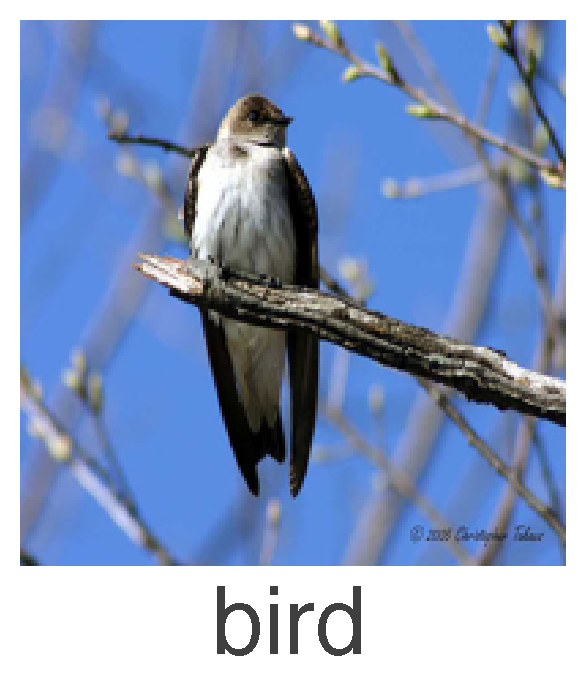
\includegraphics[height=1in]{pascal_bird.png} &
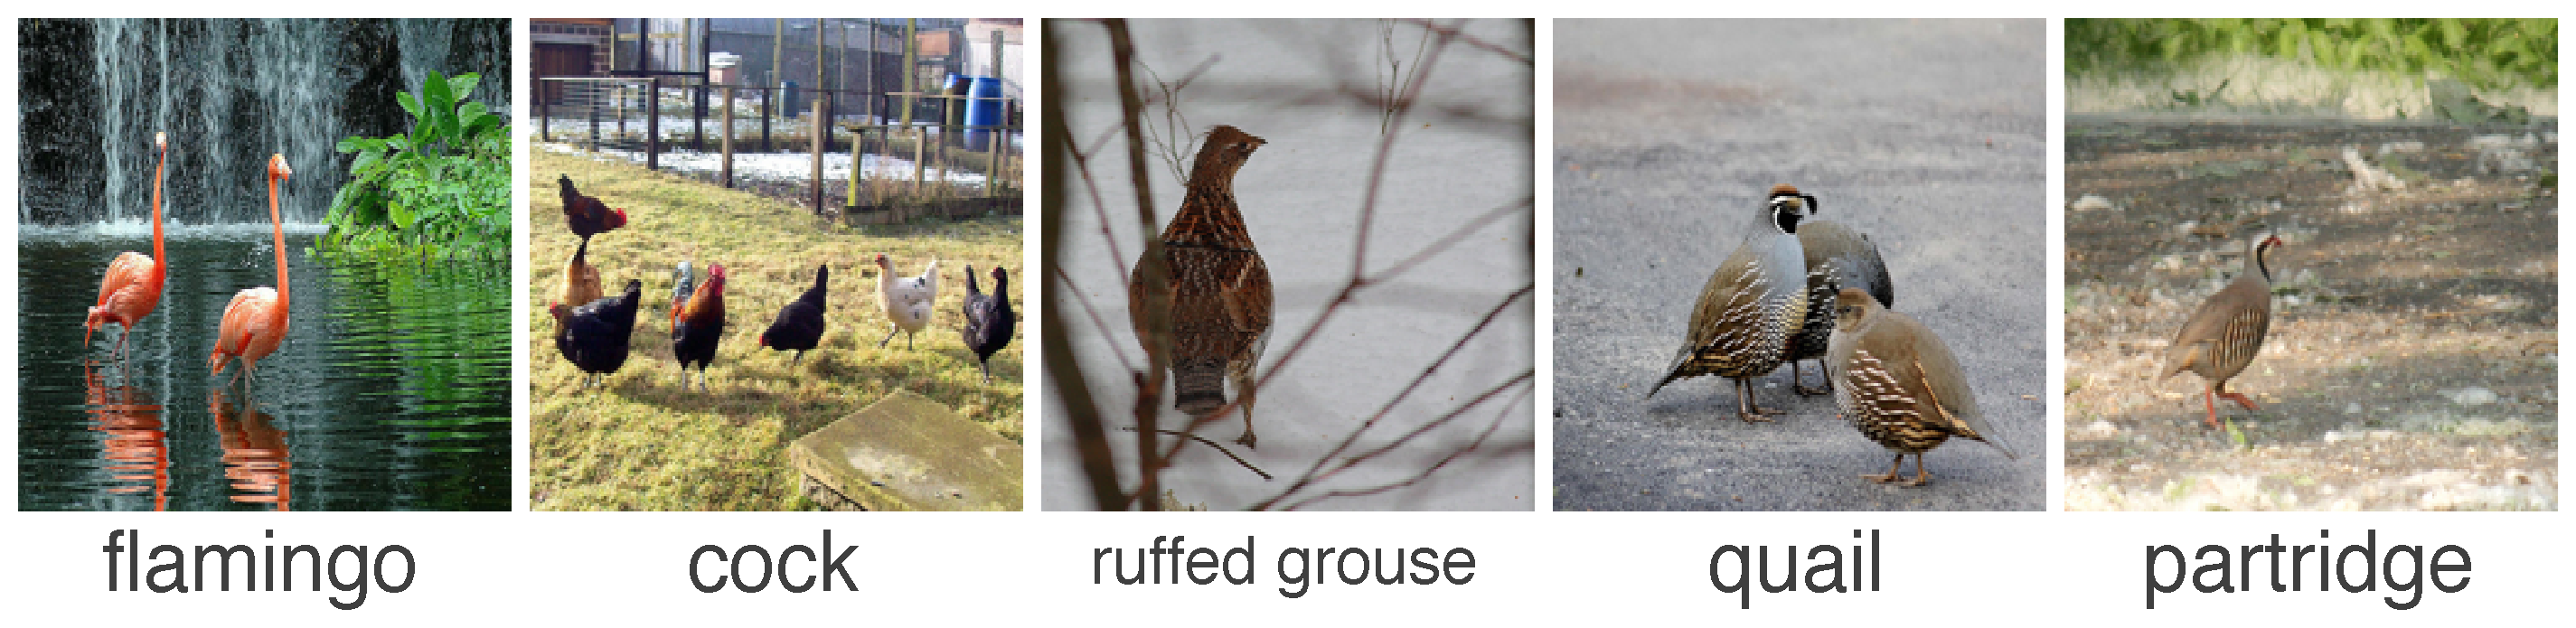
\includegraphics[height=1in]{imagenet_bird.png} $\cdots$\\
\side{1}{ cats} &
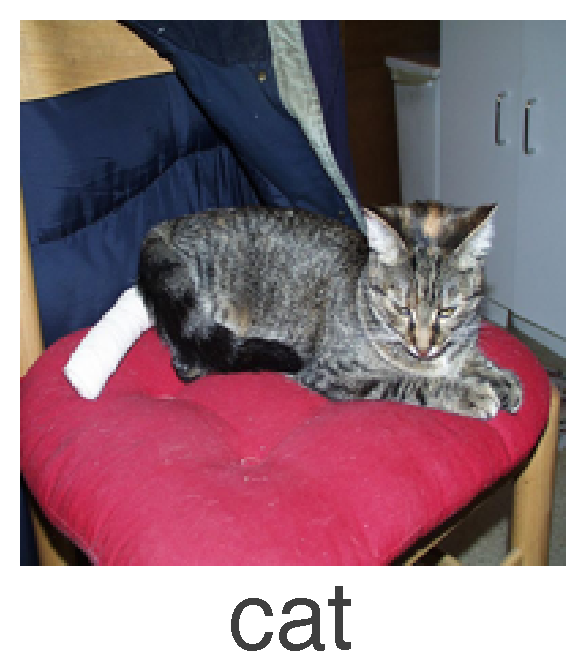
\includegraphics[height=1in]{pascal_cat.png} &
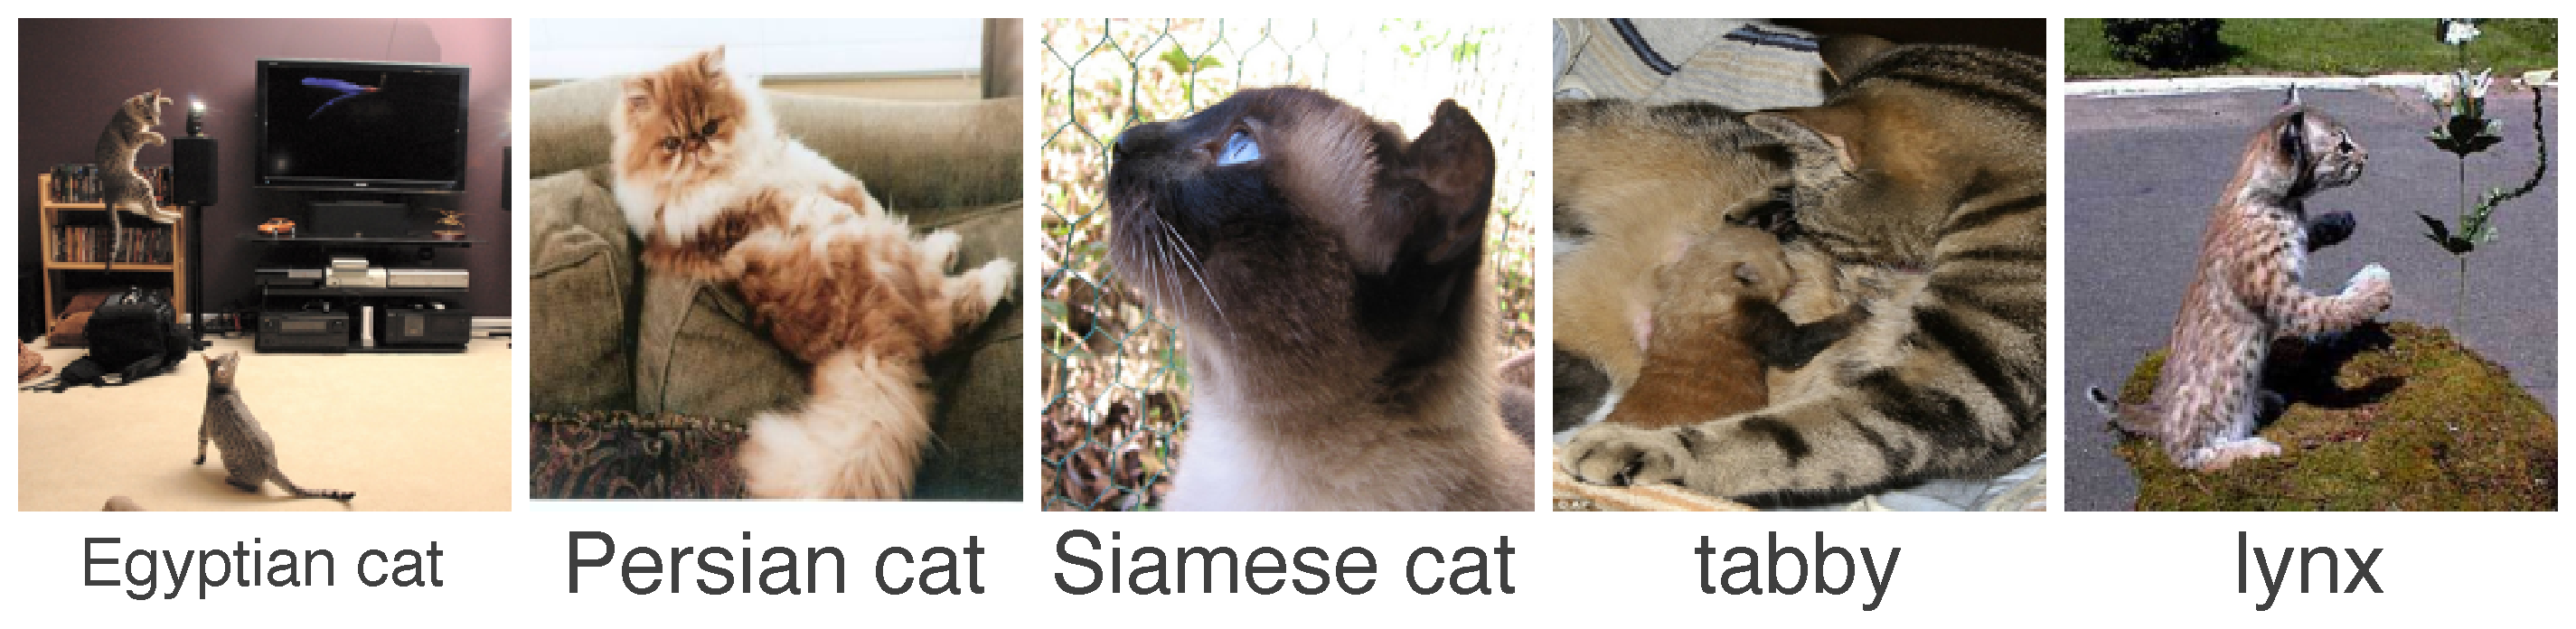
\includegraphics[height=1in]{imagenet_cat.png} $\cdots$\\
\side{1}{ dogs} &
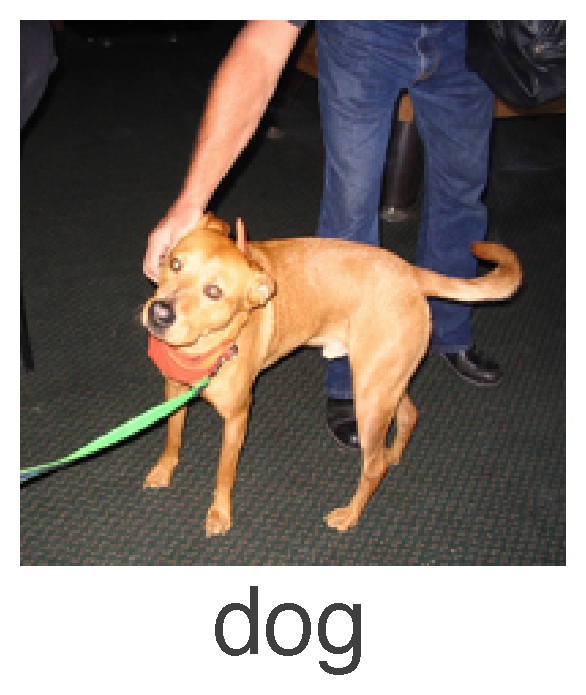
\includegraphics[height=1in]{pascal_dog.png} &
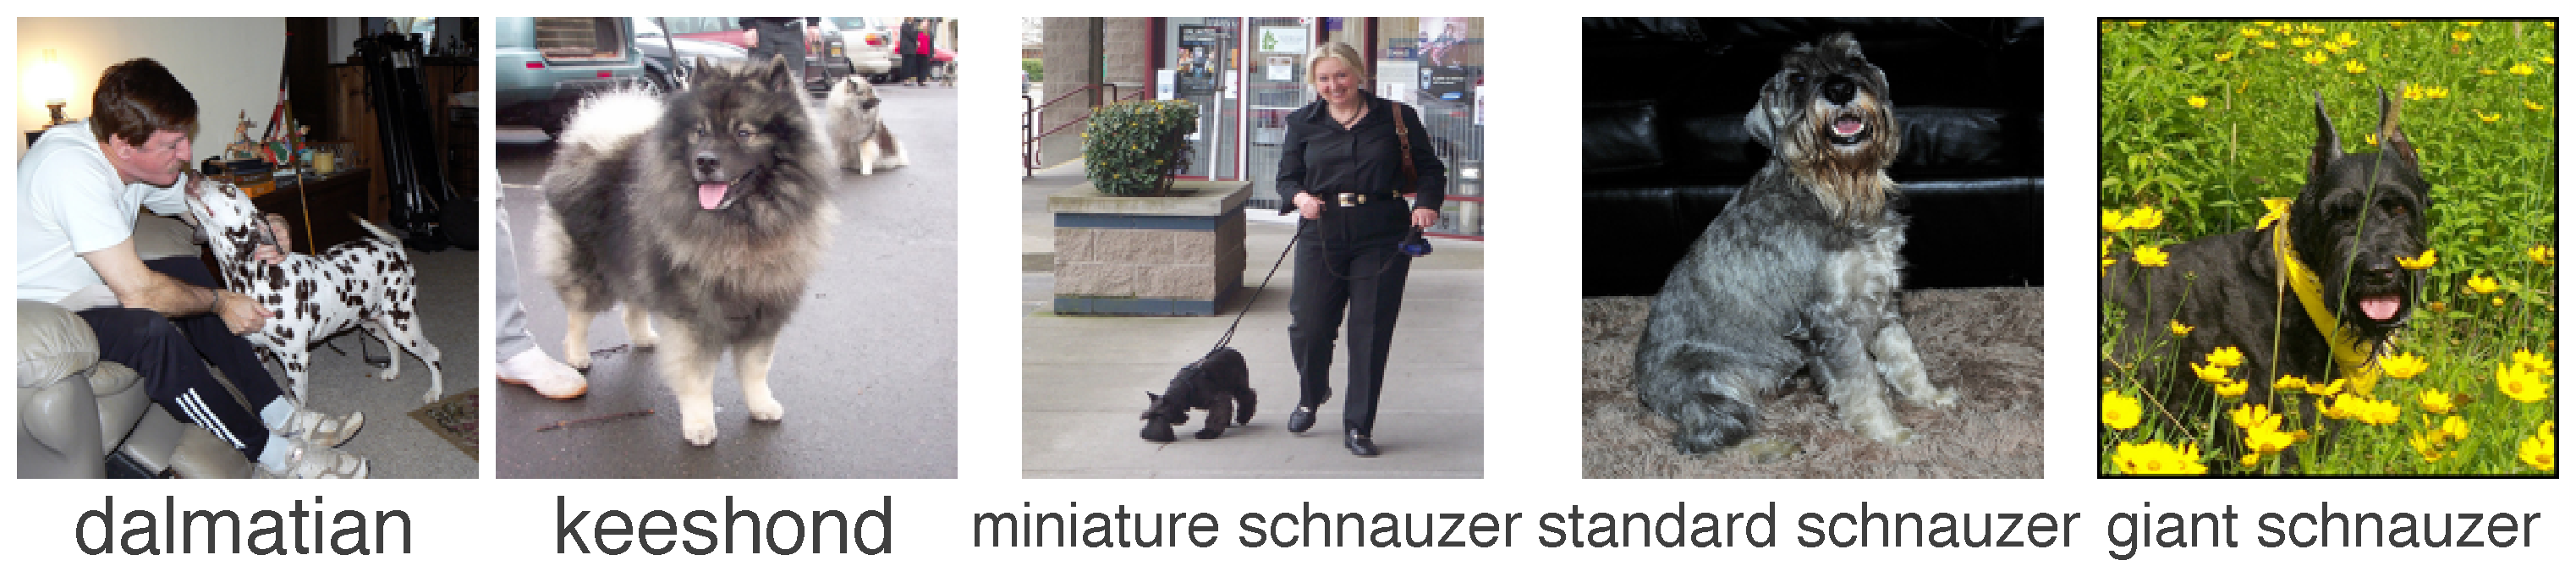
\includegraphics[height=1in]{imagenet_dog.png} $\cdots$\\
\end{tabular}
\end{center}
\caption{The ILSVRC dataset contains many more fine-grained classes compared to the standard PASCAL VOC benchmark; for example, instead of the PASCAL ``dog'' category there are 120 different breeds of dogs in ILSVRC2012-2014 classification and single-object localization tasks.}
\label{fig:fg}
\end{figure*}



\subsubsection{Collecting candidate images for the image classification dataset}
\label{sec:AnnotClsImages}

Image collection for ILSVRC classification task is the same as the strategy employed for constructing
 ImageNet~\citep{ImageNet}. Training images are taken directly from ImageNet. Additional
images are collected for the ILSVRC using this strategy and randomly partitioned into the validation and test sets.

We briefly summarize the process; \citep{ImageNet} contains further details. Candidate images are collected from the Internet by querying several image search engines. For each synset, the queries are the set of WordNet synonyms. Search engines typically limit the number of retrievable images (on the order of a few hundred to a thousand). To obtain as many images as possible, we expand the query set by appending the queries with the word from parent synsets, if the same word appears in the glossary of the target synset. For example, when querying ``whippet'', according to WordNet's glossary a ``small slender dog of greyhound type developed in England'', we also use ``whippet dog'' and ``whippet greyhound.''
To further enlarge and diversify the candidate pool, we translate the queries into other languages, including Chinese, Spanish, Dutch and Italian. We obtain accurate translations using WordNets in those languages.



\subsubsection{Image classification dataset annotation}
\label{sec:AnnotClsAnnot}

Annotating images with corresponding object classes follows the strategy employed by ImageNet~\citep{ImageNet}. We summarize it briefly here.

To collect a highly accurate dataset, we rely on humans to verify each candidate image collected in the previous step for a given synset. This is achieved by using Amazon Mechanical Turk (AMT), an online platform on which one can put up tasks for users for a monetary reward. With a global user base, AMT is particularly suitable for large scale labeling.
In each of our labeling tasks, we present the users with a set of candidate images and the definition of the target synset (including a link to Wikipedia). We then ask the users to verify whether each image contains objects of the synset. We encourage users to select images regardless of occlusions, number of objects and clutter in the scene to ensure diversity.

While users are instructed to make accurate judgment, we need to set up a quality control system to ensure this accuracy. There are two issues to consider. First, human users make mistakes and not all users follow the instructions. Second, users do not always agree with each other, especially for more subtle or confusing synsets, typically at the deeper levels of the tree. The solution to these issues is to have multiple users independently label the same image. An image is considered positive only if it gets a convincing majority of the votes. We observe, however, that different categories require different levels of consensus among users. For example, while five users might be necessary for obtaining a good consensus on “Burmese cat” images, a much smaller number is needed for “cat” images. We develop a simple algorithm to dynamically determine the number of agreements needed for different categories of images. For each synset, we first randomly sample an initial subset of images. At least 10 users are asked to vote on each of these images. We then obtain a confidence score table, indicating the probability of an image being a good image given the consensus among user votes. For each of the remaining candidate images in this synset, we proceed with the AMT user labeling until a pre-determined confidence score threshold is reached.

\paragraph{Empirical evaluation.}  Evaluation of the accuracy of the large-scale crowdsourced image annotation system was done on the entire ImageNet~\citep{ImageNet}. 
A total of 80 synsets were randomly sampled at every tree depth of
the mammal and vehicle subtrees. An independent group of subjects verified the correctness of each of the images. An average of $99.7\%$ precision is achieved across the synsets. We expect similar accuracy on ILSVRC image classification dataset since the image annotation pipeline has remained the same. To verify, we manually checked 1500 ILSVRC2012-2014 image classification test set images (the test set has remained unchanged in these three years). We found 5 annotation errors, corresponding as expected to $99.7\%$ precision.


\subsubsection{Image classification dataset statistics}
\label{sec:ClsStats}


Using the image collection and annotation procedure described in previous sections, we collected a large-scale dataset
used for ILSVRC classification task. There are 1000 object classes and approximately 1.2 million training images, 50 thousand validation images and 100 thousand test images. Table~\ref{table:clslocstats} (top) documents the size of the dataset over the years of the challenge. 

%%%%%%%%%%%%%%%%%%%%%%%%%%%%%%%%%%%%%%%%%%%%%%%%%%%%%
\begin{table*}

\begin{center} {\bf Image classification annotations (1000 object classes)} \end{center}

\begin{tabular}{|p{0.9in}|c|c|c|c|}
\hline
Year
 %&
%\parbox[t]{1in}{\centering {Object classes}}
&
\parbox[t]{2.3in}{\centering {Train images  (per class)}}
&
\parbox[t]{1.95in}{\centering {Val images  (per class)}}
&
\parbox[t]{1.25in}{\centering {Test images  (per class)}}
\\
\hline
ILSVRC2010 
&
1,261,406  (668-3047)
&
50,000  (50)
&
150,000  (150)
\\
\hline
ILSVRC2011
&
1,229,413 (384-1300)
&
50,000  (50)
&
100,000  (100)
\\
\hline
ILSVRC2012-14 
&
1,281,167  (732-1300)
&
 50,000  (50)
&
 100,000  (100)
\\
\hline
\end{tabular}


\begin{center}
{\bf Additional annotations for single-object localization (1000 object classes)}
\end{center}

\begin{tabular}{|p{0.9in}|c|c|c|c|c|c|}
\hline
Year
 %&
%\parbox[t]{0.4in}{\centering {Object \\ classes}}
&
\parbox[t]{1.1in}{\centering {Train images  with \\ bbox annotations \\ (per class)}}
&
\parbox[t]{1in}{\centering {Train bboxes\\ annotated \\ (per class)}}
&
\parbox[t]{0.95in}{\centering {Val images   with \\ bbox annotations \\ (per class)}}
&
\parbox[t]{0.8in}{\centering {Val bboxes \\annotated \\ (per class)}}
&
\parbox[t]{1.25in}{\centering {Test images  with \\ bbox annotations}}
\\
\hline
ILSVRC2011
& 315,525 (104-1256)
& 344,233 (114-1502)
& 50,000 (50)
& 55,388 (50-118)
& 100,000
\\
\hline
ILSVRC2012-14 
& 523,966 (91-1268)
& 593,173 (92-1418)
& 50,000 (50)
& 64,058 (50-189)
& 100,000
\\
\hline
\end{tabular}

\caption{Scale of ILSVRC image classification task (top) and single-object localization task (bottom). The numbers in parentheses correspond to (minimum per class - maximum per class). The 1000 classes change from year to year but are consistent between image classification and single-object localization tasks in the same year. All images from the image classification task may be used
for single-object localization.}
\label{table:clslocstats}
\end{table*}

%%%%%%%%%%

\iffalse
\begin{table}
\begin{tabular}{|p{0.8in}|c|c|c|}
\hline
Year & ILSVRC2010 & ILSVRC2011 & ILSVRC2012-14 \\
\hline
Object classes & 1000 & 1000 & 1000  \\
\hline
\parbox[t]{0.8in}{Train images \\ (per class)} &
\parbox[t]{0.7in}{\centering 1,261,406 \\ (668-3047)} &
\parbox[t]{0.7in}{\centering 1,229,413 \\ (384-1300)} &
\parbox[t]{0.7in}{\centering 1,281,167 \\ (732-1300)} 
 \\
\hline
\parbox[t]{0.8in}{Val images \\ (per class)} &
 \parbox[t]{0.7in}{\centering 50,000 \\ (50)} &
 \parbox[t]{0.7in}{\centering 50,000 \\ (50)} & 
 \parbox[t]{0.7in}{\centering 50,000 \\ (50)} 
\\
\hline
\parbox[t]{0.8in}{Test images \\ (per class)} &
 \parbox[t]{0.7in}{\centering 150,000 \\ (150)} &
 \parbox[t]{0.7in}{\centering 100,000 \\ (100)} &
 \parbox[t]{0.7in}{\centering 100,000 \\ (100)} 
\\
\hline
\end{tabular}
\fi

%%%%%%%%%%%%%%%%%%%%%%%%%%%%%%%%%%%%%%%%%%%%%%%%%%%%%

%%%%%%%%%%%%%%%%%%%%%%%%%%%%%%%%%%%%%%%%%%%%%%%%%%%%%%%%%%%%%%%%%%%%%%%%%%%%%%%%%%%%%%%%%%
%%%%%%%%%%%                                                            %%%%%%%%%%%%%%%%%%%%%%%%%%%%%%%%%%%%%%%%%%%%%%%%%%%
%%%%%%%%%%%        Localization annotation                %%%%%%%%%%%%%%%%%%%%%%%%%%%%%%%%%%%%%%%%%%%%%%%%%%%
%%%%%%%%%%%                                          	             %%%%%%%%%%%%%%%%%%%%%%%%%%%%%%%%%%%%%%%%%%%%%%%%%%%
%%%%%%%%%%%%%%%%%%%%%%%%%%%%%%%%%%%%%%%%%%%%%%%%%%%%%%%%%%%%%%%%%%%%%%%%%%%%%%%%%%%%%%%%%%

\subsection{Single-object localization dataset construction}
\label{sec:AnnotLoc}

The single-object localization task evaluates the ability of an algorithm to localize one instance of an object category.
It was introduced as a  taster task in ILSVRC 2011, and became an official part of ILSVRC in 2012.

The key challenge
was developing a scalable crowdsourcing method for object bounding box annotation. Our three-step self-verifying
pipeline is described in Section~\ref{sec:AnnotLocBbox}. Having the dataset collected, we perform detailed analysis in Section~\ref{sec:LocStats}
to ensure that the dataset is sufficiently varied to be suitable for evaluation of object localization algorithms.

\paragraph{Object classes and candidate images.}
The object classes for single-object localization task are the same as the object classes for image classification task described above in Section~\ref{sec:AnnotCls}. The training
images for localization task are a subset of the training images used for image classification task, and the validation and test
images are the same between both tasks. 

%Details on image collection and on annotation of each image
%with one object class are in Section~\ref{sec:AnnotClsImages} and Section~\ref{sec:AnnotClsAnnot} respectively.


%In this section we discuss the bounding box annotation procedure, and provide statistics of the single-object localization dataset.

\paragraph{Bounding box annotation.} Recall that for the image classification task every image was annotated with one object class label, corresponding to
one object that is present in an image. For the single-object localization task, every validation and test image and a subset of the training images
are annotated with axis-aligned bounding boxes around every instance of this object.

Every bounding box is required to be as small as possible while including all visible parts of the object instance. An alternate annotation procedure could be to annotate the \emph{full (estimated) extent} of the object: e.g., if a person's legs are occluded and only the torso is visible, the bounding box could be drawn to include the likely location of the legs. However, this alternative procedure is inherently ambiguous and ill-defined, leading to disagreement among annotators and among researchers (what is the true ``most likely'' extent of this object?). We follow the standard protocol of only annotating visible object parts~\citep{LabelMe,PASCALIJCV}.\footnote{Some datasets such as PASCAL VOC~\citep{PASCALIJCV} and LabelMe~\citep{LabelMe} are able to provide more detailed annotations: for example, marking individual object instances as being \emph{truncated}. We chose not to provide this level of detail in favor of annotating more images and more object instances.}

\subsubsection{Bounding box object annotation system}
\label{sec:AnnotLocBbox}

We summarize the crowdsourced bounding box annotation system described in detail in~\citep{Su12}. The goal is to build a system that is fully automated, highly accurate, and cost-effective. Given a collection of images where the object of interest has been verified to exist, for each image the system collects a tight bounding box for every instance of the object. 

There are two requirements:

\begin{itemize}
\item {\bf Quality} Each bounding box needs to be tight, i.e. the smallest among all bounding boxes that contains all visible parts of the object. This facilitates the object detection learning algorithms by providing the precise location of each object instance;
\item {\bf Coverage} Every object instance needs to have a bounding box. This is important for training localization algorithms because it tells the learning algorithms with certainty what is not the object. 
\end{itemize}

The core challenge of building such a system is  effectively controlling the data quality with minimal cost. Our key observation is that drawing a bounding box is significantly more difficult and time consuming than giving answers to multiple choice questions. Thus quality control through additional verification tasks is more cost-effective than consensus-based algorithms. This leads to the following workflow with simple basic subtasks:

\begin{enumerate}
\item {\bf Drawing} A worker draws one bounding box around one instance of an object on the given image.
\item {\bf Quality verification} A second worker checks if the bounding box is correctly drawn.
\item {\bf Coverage verification} A third worker checks if all object instances have bounding boxes.
\end{enumerate}

 The sub-tasks are designed following two principles. First, the tasks are made as simple as possible. For example, instead of asking the worker to draw all bounding boxes on the same image, we ask the worker to draw only one. This reduces the complexity of the task. Second, each task has a fixed and predictable amount of work. For example, assuming that the input images are clean (object presence is correctly verified) and the coverage verification tasks give correct results, the amount of work of the drawing task is always that of providing exactly one bounding box.

Quality control on Tasks 2 and 3 is implemented by embedding ``gold standard'' images where the correct answer is known. Worker training for each of these subtasks is described in detail in~\citep{Su12}.

\paragraph{Empirical evaluation.} The system is evaluated on 10 categories with ImageNet~\citep{ImageNet}:  balloon, bear, bed, bench, beach, bird, bookshelf, basketball hoop, bottle, and people. A subset of 200 images are randomly sampled from each category. On the image level, our evaluation shows that $97.9\%$ images are completely covered with bounding boxes. For the remaining $2.1\%$, some bounding boxes are missing. However, these are all difficult cases: the size is too small, the boundary is blurry, or there is strong shadow.

On the bounding box level, $99.2\%$ of all bounding boxes are accurate (the bounding boxes are visibly tight). The remaining $0.8\%$ are somewhat off. No bounding boxes are found to have less than $50\%$ intersection over union overlap with ground truth.

Additional evaluation of the overall cost and an analysis of quality control can be found in~\citep{Su12}.


%\todo{ annotate all (up to N) instances in the image with bboxes; examples critical for more complicated objects; pictures %from Hao's paper}

\subsubsection{Single-object localization dataset statistics}
\label{sec:LocStats}

Using the annotation procedure described above, we collect a large set of bounding box annotations
for the ILSVRC single-object classification task. All 50 thousand images in the validation set and
100 thousand images in the test set are annotated with bounding boxes around all instances of the
ground truth object class (one object class per image). In addition, in ILSVRC2011 
$25\%$ of training images are annotated with bounding boxes the same way, yielding more than 310 thousand
annotated images with more than 340 thousand annotated object instances. In ILSVRC2012 $40\%$ of
training images are annotated, yielding more than 520 thousand 
annotated images with more than 590 thousand annotated object instances. 
Table~\ref{table:clslocstats} (bottom) documents the size of this dataset.

In addition to the size of the dataset, we also analyze the level of difficulty of object localization
in these images compared to the PASCAL VOC benchmark. We compute statistics on the ILSVRC2012 single-object localization
validation set images compared to PASCAL VOC 2012 validation images. 

Real-world scenes are likely to contain multiple instances of some objects, and nearby object instances are particularly difficult to delineate.  The average object category in ILSVRC has $1.61$ target object instances on average per positive image, with each instance having on average $0.47$ neighbors (adjacent instances of the same object category). This is comparable to $1.69$ instances per positive image and $0.52$ neighbors per instance for an average object class in PASCAL. 

As described in~\citep{Hoiem12}, smaller objects tend to be significantly more difficult to localize. In the average object category in PASCAL
the object occupies $24.1\%$ of the image area, and in ILSVRC $35.8\%$. However, PASCAL has only 20 object
categories while ILSVRC has 1000. The 537 object categories of ILSVRC with the smallest objects on average occupy the same
fraction of the image as PASCAL objects: $24.1\%$. Thus even though on average the object instances tend to be bigger in ILSVRC images,
there are more than 25 times more object categories than in PASCAL VOC with the same average object scale. 

Appendix~\ref{app:ICCV} and~\citep{Russakovsky13} have additional comparisons. 





%%%%%%%%%%%%%%%%%%%%%%%%%%%%%%%%%%%%%%%%%%%%%%%%%%%%%%%%%%%%%%%%%%%%%%%%%%%%%%%%%%%%%%%%%%
%%%%%%%%%%%                                                            %%%%%%%%%%%%%%%%%%%%%%%%%%%%%%%%%%%%%%%%%%%%%%%%%%%
%%%%%%%%%%%        Detection annotation                   %%%%%%%%%%%%%%%%%%%%%%%%%%%%%%%%%%%%%%%%%%%%%%%%%%%
%%%%%%%%%%%                                          	             %%%%%%%%%%%%%%%%%%%%%%%%%%%%%%%%%%%%%%%%%%%%%%%%%%%
%%%%%%%%%%%%%%%%%%%%%%%%%%%%%%%%%%%%%%%%%%%%%%%%%%%%%%%%%%%%%%%%%%%%%%%%%%%%%%%%%%%%%%%%%%

\subsection{Object detection dataset construction}
\label{sec:AnnotDet}

The ILSVRC task of object detection evaluates the ability of an algorithm to name and localize \emph{all} instances
of \emph{all} target objects present in an image. It is much more challenging than object localization because
some object instances may be small/occluded/difficult to accurately localize, and the algorithm is expected
to locate them all, not just the one it finds easiest. 

%The image collection and annotation procedures for this task are different than for either image classification or
%single-object localization. The images are chosen to be more scene-like, and annotating in a straight-forward
%way by creating a task for every (image, object class) pair is no longer feasible.

There are three key challenges in collecting the object detection dataset.
The first challenge is selecting the set of common objects which tend to appear in cluttered photographs
and are well-suited for benchmarking object detection performance. Our approach relies 
on statistics of the object localization dataset and the tradition of the
PASCAL VOC challenge (Section~\ref{sec:AnnotDetObjects}). 

The second challenge is obtaining a much more varied set of scene images than those used for
the image classification and single-object localization datasets. Section~\ref{sec:AnnotDetImages} describes the
procedure for utilizing as much data from the single-object localization dataset as possible and supplementing it with
Flickr images queried using hundreds of manually designed high-level queries.

The third, and biggest, challenge is 
completely annotating this dataset with all the objects. 
This is done in two parts. Section~\ref{sec:AnnotDetList} describes the first part: 
our hierarchical strategy for obtaining the list of all target objects which occur within every image. This is necessary since annotating in a straight-forward way by creating a task for every (image, object class) pair is no longer feasible at this scale. 
Appendix~\ref{sec:AppDetBbox} describes the second part: annotating the bounding boxes around these objects, using the single-object localization bounding box annotation pipeline of Section~\ref{sec:AnnotLocBbox} along with extra verification to ensure that \emph{every} instance of the object is annotated with exactly \emph{one} bounding box.


\subsubsection{Defining object categories for the object detection dataset}
\label{sec:AnnotDetObjects}

\begin{table}[t]
\centering
\begin{tabular}{|l|l| c| c|}
\hline
Class name in &  Closest class in & \multicolumn{2}{c|}{Avg object scale (\%)} \\
\cline{3-4}
PASCAL VOC & ILSVRC-DET & PASCAL & ILSVRC- \\
{\bf (20 classes)} & {\bf (200 classes)} & VOC & DET\\


%{\bf PASCAL VOC (20) } & {\bf Closest ILSVRC-DET (200)} \\
%PASCAL VOC class & Closest of ILSVRC-DET classes \\
\hline
aeroplane & airplane & 29.7 & 22.4\\
\hline
bicycle & bicycle & 29.3 & 14.3 \\
\hline
bird & bird & 15.9 & 20.1 \\
\hline
\emph{boat} & \emph{watercraft} & 15.2 & 16.5 \\
\hline
\emph{bottle} & \emph{wine bottle} & 7.3 & 10.4\\
\hline
bus & bus & 29.9 & 22.1 \\
\hline
car & car & 14.0 & 13.4\\
\hline
cat & domestic cat & 46.8 & 29.8 \\
\hline
chair & chair  & 12.8 & 10.1 \\
\hline
\emph{cow} & \emph{cattle} & 19.3 & 13.5 \\
\hline
\emph{dining table} & \emph{table} & 29.1 & 30.3 \\
\hline
dog & dog & 37.0 & 28.9 \\
\hline
horse & horse & 29.5 & 18.5 \\
\hline
motorbike & motorcyle& 32.0 & 20.7 \\
\hline
person & person & 17.5 & 19.3 \\
\hline
\emph{potted plant} & \emph{flower pot} & 12.3 & 8.1\\
\hline
sheep & sheep & 12.2 & 17.3 \\
\hline
sofa & sofa & 41.7 & 44.4 \\
\hline
train & train  & 35.4 & 35.1\\
\hline
tv/monitor & tv or monitor & 14.6 & 11.2\\
\hline
\end{tabular}
\caption{Correspondences between the object classes in the PASCAL VOC~\citep{PASCALIJCV} and the ILSVRC detection task.
Object scale is the fraction of image area (reported in percent) occupied by an object instance. It is computed on the validation sets of
PASCAL VOC 2012 and of ILSVRC-DET. The average object scale is $24.1\%$  across the 20 PASCAL VOC categories 
and $20.3\%$ across the 20 corresponding ILSVRC-DET categories. Section~\ref{sec:AnnotDetStats} reports additional dataset statistics.
%In addition, ILSVRC-DET has 10x more object classes than PASCAL VOC 
%and 3.5x more training instances on average per class (680 in PASCAL VOC 2012 versus 2394 in ILSVRC-DET 2014). 
}
\label{table:detclassespascal}
\end{table}




There are 200 object classes hand-selected for the detection task, eacg corresponding to a synset within ImageNet. 
These were chosen to be mostly basic-level object categories that would be easy for
people to identify and label. The rationale is that the object detection system developed for this task
can later be combined with a fine-grained classification model to further classify the objects if a finer
subdivision is desired.\footnote{Some of the training objects are actually annotated with more detailed classes:
for example, one of the 200 object classes is the category ``dog,'' and some training instances
are annotated with the specific dog breed.}
As with the 1000 classification classes, the synsets are selected such that there is no overlap:  for any synsets $i$ and $j$, $i$ is not an ancestor of $j$ in the ImageNet hierarchy. 

\iffalse 
\begin{figure}
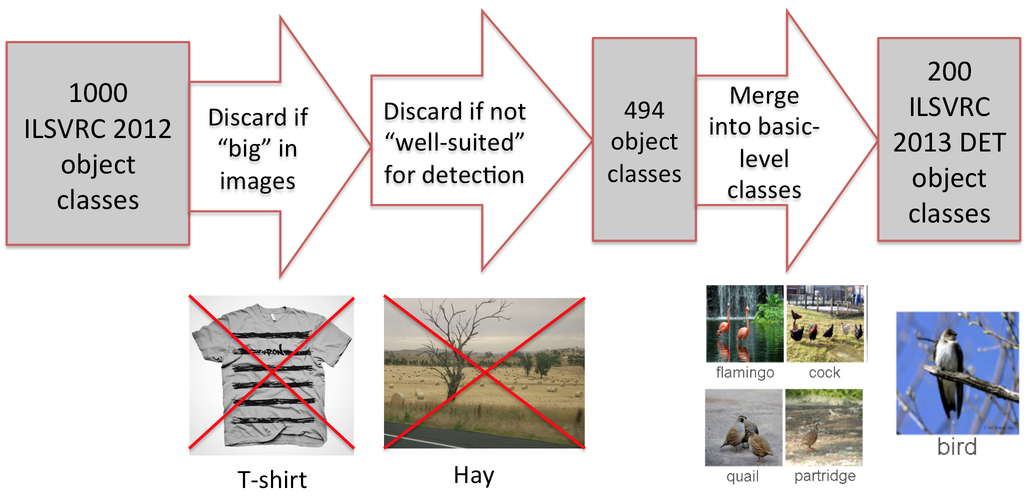
\includegraphics[width=\linewidth]{detannotpipeline.png}
\caption{Selection of 200 object classes for the detection task.}
\label{fig:detannot}
\end{figure}
\fi

The selection of the 200 object detection classes in 2013 was guided by the ILSVRC 2012 classification and localization dataset.
 Starting with 1000 object classes and their bounding box annotations we
first eliminated all object classes which tended to be too ``big'' in the image (on average the object area was greater than $50\%$ of the
image area). These were classes such as T-shirt, spiderweb, or manhole cover. We then manually eliminated all classes
which we did not feel were well-suited for detection, such as hay, barbershop, or poncho. This left 494 object classes
which were merged into basic-level categories: for example, different species of birds were merged into just the ``bird'' class.
The classes remained the same in ILSVRC2014.
Appendix~\ref{app:hierarchy} contains the complete list of object categories used in ILSVRC2013-2014 (in the context of the hierarchy described in Section~\ref{sec:AnnotDetList}).

\iffalse

\begin{figure}
\caption{200 object classes of the object detection task. \todo{THIS FIGURE}}
\label{fig:detclasses}
\end{figure}
\fi
Staying mindful of the tradition of the PASCAL VOC dataset we also tried to ensure that the set of 200 classes contains
as many of the 20 PASCAL VOC classes as possible. Table~\ref{table:detclassespascal} shows the correspondences. 
The changes that were done were to ensure more accurate and consistent crowdsourced annotations.
The object class with the
weakest correspondence is ``potted plant'' in PASCAL VOC, corresponding to  ``flower pot''  in ILSVRC. ``Potted plant'' was  one
of the most challenging object classes to annotate consistently among the PASCAL VOC classes, and in order to obtain accurate  annotations using crowdsourcing we had to restrict the definition to a more concrete object. 




\subsubsection{Collecting images for the object detection dataset}
\label{sec:AnnotDetImages}

\begin{figure}[t]
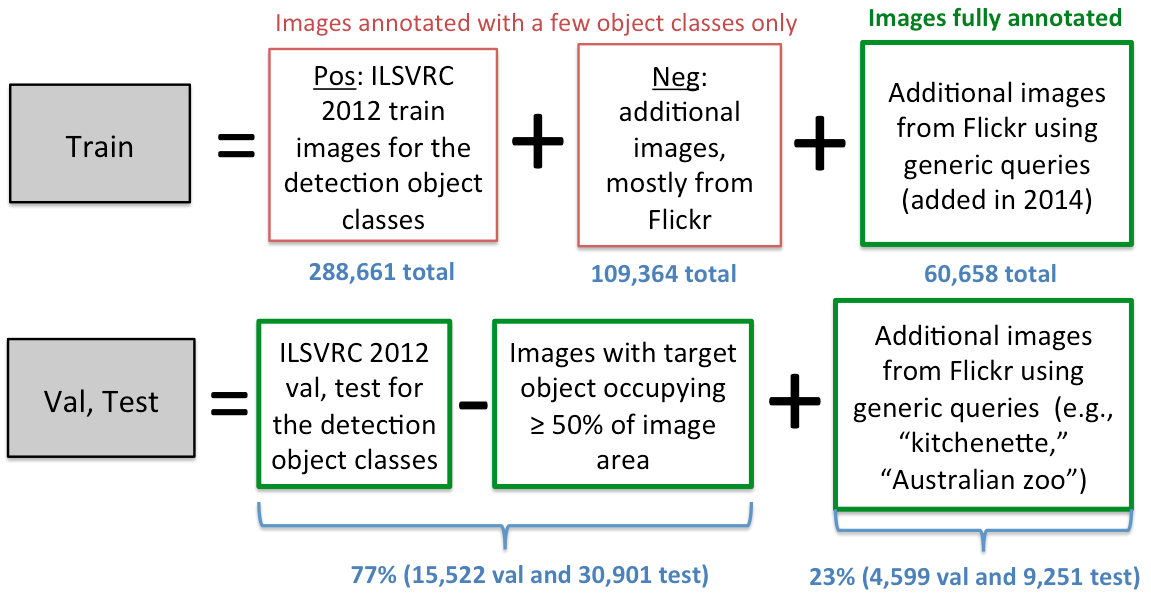
\includegraphics[width=\linewidth]{detdata.png}
\caption{Summary of images collected for the detection task. Images in green (bold) boxes have all instances of all 200 detection object classes fully annotated. Table~\ref{table:detstats} lists the complete statistics.}
\label{fig:detsummary}
\end{figure}

Many images for the detection task were collected differently than the images in ImageNet and the classification and single-object
localization tasks. Figure~\ref{fig:detsummary} summarizes the types of images that were collected. Ideally all of these images would be scene images fully annotated with all target categories. However, given budget constraints our goal was to provide as much suitable detection data as possible, even if the images were drawn from a few different sources and distributions.

The validation and test detection set images come from two sources (percent of images from each source in parentheses).
The first source $(77\%)$ is images from ILSVRC2012 single-object localization validation and test sets
corresponding to the 200 detection classes (or their children in the ImageNet hierarchy). 
Images where the target object occupied more than $50\%$ of the image area were discarded, since they were unlikely to contain
other objects of interest. The second source $(23\%)$ is images from Flickr collected specifically for detection task. We queried Flickr using a large set of manually defined queries, such as ``kitchenette'' or ``Australian zoo'' to retrieve images of scenes likely to contain
several objects of interest. Appendix~\ref{sec:AppQueries} contains the full list. We also added pairwise queries, or queries with two target object names such as ``tiger lion,'' which also often returned cluttered
scenes. 

\begin{figure*}
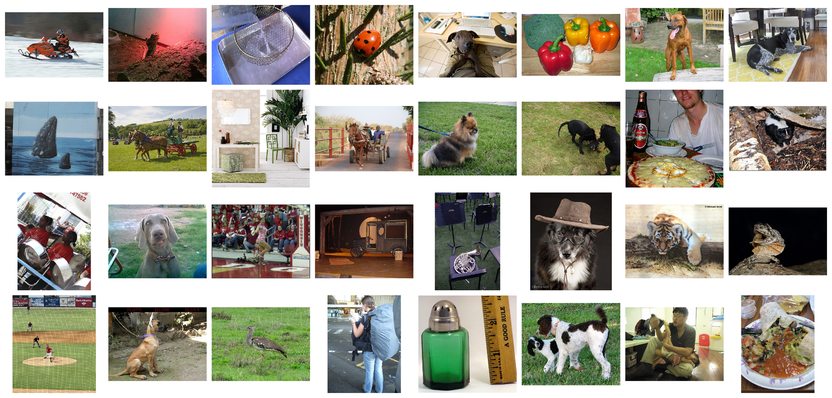
\includegraphics[width=\linewidth]{det_val_2012.png}
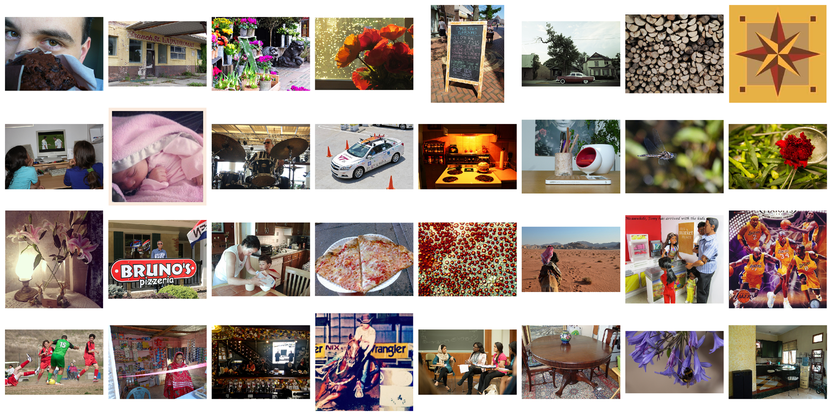
\includegraphics[width=\linewidth]{det_val_2013.png}
\caption{Random selection of images in ILSVRC detection validation set. The images in the top 4 rows were taken from ILSVRC2012 single-object localization
validation set, and the images in the bottom 4 rows were collected from Flickr using scene-level queries.}
\label{fig:detimgs}
\end{figure*}

 Figure~\ref{fig:detimgs} shows a random set of both types of validation images. Images were randomly split, with $33\%$ going into the validation set and $67\%$ into the test set.\footnote{The validation/test split is consistent with ILSVRC2012:
validation images of ILSVRC2012 remained in the validation set of ILSVRC2013, and ILSVRC2012 test images remained in ILSVRC2013 test set.}
% In total there are $20,121$ validation and $40,152$ test images.

The training set for the detection task comes from three sources of images (percent of images from each source in parentheses). 
The first source $(63\%)$ is all training images from ILSVRC2012 single-object localization task corresponding
to the 200 detection classes (or their children in the ImageNet hierarchy). We did not filter by object size, allowing teams to take advantage of all the
positive examples available. The second source $(24\%)$ 
is negative images which were part of the original ImageNet collection process but voted as negative:
for example, some of the images were collected from Flickr and search engines for the ImageNet synset ``animals'' but during the manual
verification step did not collect enough votes to be considered as containing an ``animal.'' These images were manually re-verified for the detection task 
to ensure that they did not in fact contain the target objects.  The third source $(13\%)$ is images collected from Flickr specifically for the detection task. These images were added for ILSVRC2014 following the same protocol
as the second type of images in the validation and test set. This was done to bring the training and testing distributions closer together.



%In total there are 288,661 training images from the ILSVRC2012 single-object localization task (between 417 and 66,991 per class), 109,364 additional 
%annotated negative training images (185-10,073 per class) and 60,658 Flickr scene images added in ILSVRC2014.


%One of the big challenges in collecting images for the detection task was getting enough diversity in the data. For example, for small hand-held tools
%such as screwdrivers the photos tend to either be closeup ``product'' shots of the objects or scenes where the object is barely visible \todo{Figure?}.


%\todo{collection in ILSVRC2013 vs 2014: 2013 rely heavily on cluttered pictures from localization dataset + collect more from Flickr  using pairwise queries; training distribution different from test distribution which is bad; %2014 entirely collected from Flickr; reaching limits of images with small cluttered screwdrivers}





\subsubsection{Complete image-object annotation for the object detection dataset}
\label{sec:AnnotDetList}

The key challenge in annotating images for the object detection task is that all objects in all images need to be labeled. 
Suppose there are N inputs (images) which need to be annotated with the presence or absence of K labels (objects). A na\"ive approach would query humans for each combination of input and label, requiring $NK$ queries. However,  N and K can be very large and the cost of this exhaustive approach quickly becomes prohibitive. For example, annotating $60,000$ validation and test images with the presence or absence of $200$ object classes for the detection task na\"ively would take $80$ times more effort than
annotating $150,000$ validation and test images with $1$ object each for the classification task -- and this is not even counting the additional cost of collecting bounding box annotations around each object instance.  This quickly becomes infeasible. 

In~\citep{Deng14} we study strategies for scalable multilabel annotation, or for efficiently acquiring multiple labels from humans for a collection of items. 
We exploit three key observations for labels in real world applications (illustrated in Figure~\ref{fig:chipull}):

\begin{figure}
\flushright
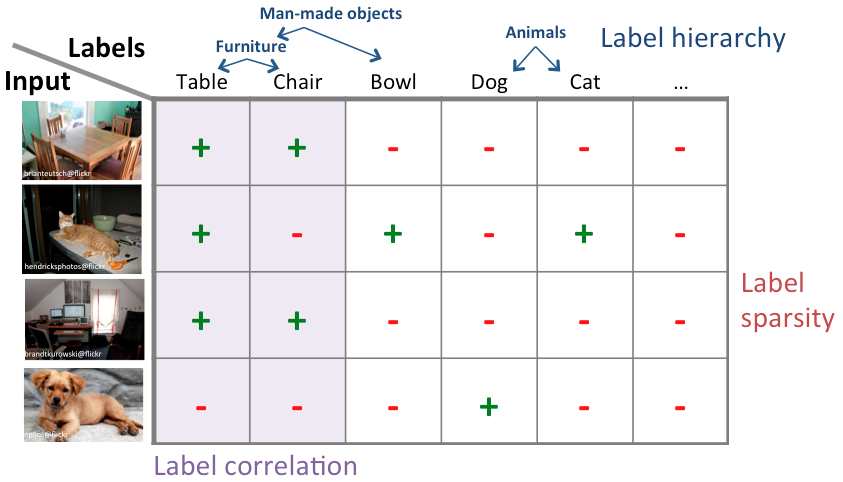
\includegraphics[width=3.25in]{chi_pullfig.png}
\caption{Consider the problem of binary multi-label annotation. For each input (e.g., image) and each label (e.g., object), the goal is to determine the presence or absense (+ or -) of the label (e.g., decide if the object is present in the image). Multi-label annotation becomes much more efficient when considering real-world structure of data: correlation between labels, hierarchical organization of concepts, and sparsity of labels.}
\label{fig:chipull}
\end{figure}

\begin{enumerate}
\item {\bf Correlation.} Subsets of labels are often highly correlated. Objects such as a computer keyboard, mouse and monitor frequently co-occur  in images. Similarly, some labels tend to all be absent at the same time. For example, all objects that require electricity are usually absent in pictures taken outdoors. This suggests that we could potentially “fill in” the values of multiple labels by grouping them into only one query for humans. Instead of checking if dog, cat, rabbit etc. are present in the photo, we just check about the ``animal'' group If the answer is no, then this implies a no for all categories in the group.

\item {\bf Hierarchy.} The above example of grouping dog, cat, rabbit etc. into animal has implicitly assumed that labels can be
grouped together and humans can efficiently answer queries about the group as a whole. This brings up our second key observation: humans organize semantic concepts into hierarchies and are able to efficiently categorize at higher semantic levels~\citep{Thorpe96}, e.g. humans can determine the presence of an animal in an image as fast as every type of animal individually. This leads to substantial cost savings.

\item {\bf Sparsity.} The values of labels for each image tend to be sparse, i.e. an image is unlikely to contain more than a dozen types of objects, a small fraction of the hundreds of object categories. This enables rapid elimination of many objects by quickly filling in no. With a high degree of sparsity, an efficient algorithm can have a cost which grows logarithmically with the number of objects instead of linearly.
\end{enumerate}



We propose algorithmic strategies that exploit the above intuitions. The key is to select a sequence of queries for humans such that we achieve the same labeling results with only a fraction of the cost of the na\"ive approach. The main challenges include how to measure cost and utility of queries, how to construct good queries, and how to dynamically order them. A detailed description of the generic algorithm, along with theoretical analysis and empirical evaluation, is presented in~\citep{Deng14}.  

%Here we discuss the simplified version of this algorithm used for labeling images for ILSVRC detection task. 


\paragraph{Application of the generic multi-class labeling algorithm to our setting.}
The generic algorithm automatically selects the most informative queries to ask based on object label statistics learned from the training set.
In our case of 200 object classes, since obtaining the training set was by itself challenging we chose to design the queries by hand.
We created a hierarchy of queries of the type ``is there a... in the image?'' For example, one of the high-level questions was ``is there an animal in the image?'' We ask the crowd workers this question about every image we want to label. 
The children of the ``animal'' question would correspond to specific examples of animals: for example, ``is there a mammal in the image?'' or ``is there an animal with no legs?'' To annotate images efficiently, these questions are asked only on images determined to contain an animal.
The 200 leaf node questions correspond to the 200 target objects, e.g., ``is there a cat in the image?''. A few sample iterations of the algorithm are shown in Figure~\ref{fig:chipipeline}. 

\begin{figure}
\centering
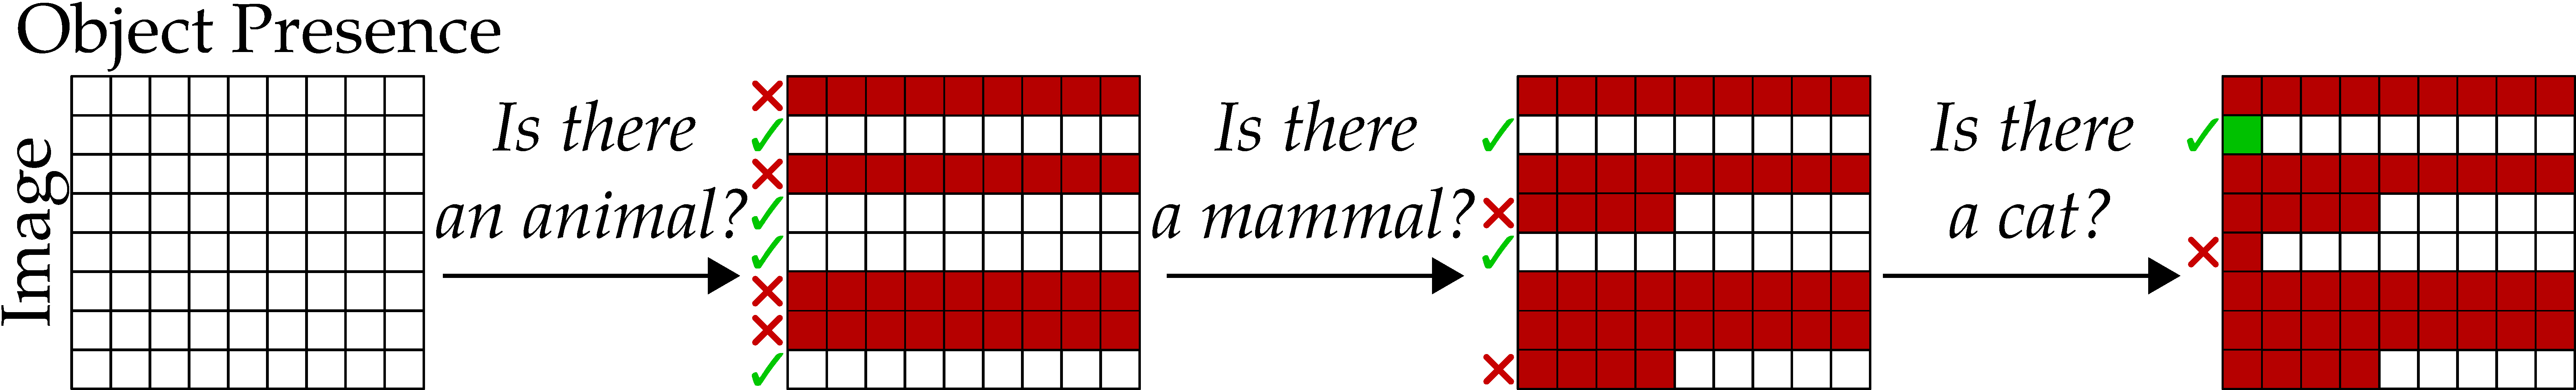
\includegraphics[width=3.35in]{chi_pipeline.pdf}
\caption{Our algorithm dynamically selects the next query to efficiently determine the presence or absence of every object in every image. Green denotes a positive annotation and red denotes a negative annotation. This toy example illustrates a sample progression of the algorithm for one label (cat) on a set of images. }
\label{fig:chipipeline}
\end{figure}




Algorithm~\ref{algorithm:chi} is the formal algorithm for labeling an image with the presence or absence of each target object category.
With this algorithm in mind, the hierarchy of questions was constructed following the principle that false positives
 only add extra cost whereas false
negatives can significantly affect the quality of the labeling. Thus, it is always better to stick with 
more general but less ambiguous questions, such as ``is there a mammal in the image?'' as opposed
to asking
overly specific but potentially ambiguous questions, such as ``is there an animal that can climb trees?''
Constructing this hierarchy was a surprisingly time-consuming process, involving multiple iterations to ensure high accuracy of labeling and avoid question ambiguity. Appendix~\ref{app:hierarchy} shows the constructed hierarchy.

%Figure~\ref{fig:qhierarchy} shows the constructed hierarchy. 
%This was a 




\paragraph{Bounding box annotation.} 
Once all images are labeled with the presence or absence of all object categories we use the bounding box 
system described in Section~\ref{sec:AnnotLocBbox}
along with some additional modifications of Appendix~\ref{sec:AppDetBbox}
 to annotate the location of every instance of every present object category.


\begin{algorithm}[t]
 \SetAlgoLined
 \KwIn{Image $i$, queries $\mathcal{Q}$, directed graph $\mathcal{G}$ over $\mathcal{Q}$}
 \KwOut{Labels $L: \mathcal{Q} \rightarrow \{$``yes'', ``no''$\}$}
Initialize labels $L(q) = \emptyset \; \forall q \in \mathcal{Q}$\;
Initialize candidates $C = \{q \mbox{: } q \in Root(\mathcal{G})\}$\;
\While{$C$ not empty}{
Obtain answer $A$ to query $q* \in C$\;
$L(q*) = A$; $C  = C \backslash \{q*\}$\;
\uIf{A is ``yes''}{
$Chldr = \{q \in Children(q*,\mathcal{G}) \mbox{: } L(q) = \emptyset \}$\;
$C = C \cup Chldr$\;
}
\Else{
$Des = \{q \in Descendants(q*,\mathcal{G}) \mbox{: } L(q) = \emptyset \}$\;
$L(q) =``no'' \; \forall q \in Des$\;
$C = C \backslash Des$\;
}
 }

 \caption{The algorithm for complete multi-class annotation. This is a special case of the algorithm described in~\citep{Deng14}.
A hierarchy of questions  $\mathcal{G}$ is manually constructed.  All root questions are asked on every image. If the answer to query $q*$ on image $i$ is ``no'' then the answer is assumed to be ``no''  for all queries $q$ such that $q$ is a descendant of $q*$ in the hierarchy. We continue asking the queries until all queries are answered. For images
taken from the single-object localization task we used the known object label to initialize $L$.
}
 \label{algorithm:chi}
\end{algorithm}

% described in Appendix~\ref{sec:AppDetLocExt}. 





%\subsubsection{Bounding box annotation}
%\label{sec:DetBbox}



\subsubsection{Object detection dataset statistics}
\label{sec:AnnotDetStats}



Using the procedure described above, we collect a large-scale dataset
for ILSVRC object detection task. 
 There are 200 object classes and approximately 450K training images, 20K validation images and 40K test images. Table~\ref{table:detstats} documents the size of the dataset over the years of the challenge. The major change between ILSVRC2013 and ILSVRC2014 was the addition of 60,658 
fully annotated training images.

Prior to ILSVRC, the object detection benchmark was the PASCAL VOC challenge~\citep{PASCALIJCV}. 
ILSVRC has $10$ times more object classes than PASCAL VOC (200 vs 20), $10.6$ times more fully annotated training images (60,658 vs 5,717), $35.2$ times more training objects (478,807 vs 13,609),
$3.5$ times more validation images (20,121 vs 5823) and $3.5$ times more validation objects (55,501 vs 
15,787). ILSVRC has $2.8$ annotated objects per image on the validation set, compared to $2.7$ in PASCAL VOC. The average object in ILSVRC takes up $17.0\%$ of the image area and in PASCAL VOC takes up $20.7\%$; Table~\ref{table:detclassespascal} contains per-class comparisons. Additionally, ILSVRC contains a wide variety of objects, including tiny objects such as sunglasses ($1.3\%$ of image area on average), ping-pong balls ($1.5\%$ of image area on average) and basketballs ($2.0\%$ of image area on average). 

%\footnote{In the average object category, the average object instance occupies $16.0\%$ of the image area in the ILSVRC detection dataset, $24.1\%$ of the image area in PASCAL VOC 2012, and $35.8\%$ of the image area in ILSVRC2012 localization validation dataset.}

\begin{table*}

\begin{center} {\bf Object detection annotations (200 object classes)} \end{center}

\begin{tabular}{|p{0.7in}|c|c|c|c|c|}
\hline
Year
 &
\parbox[t]{1.3in}{\centering {Train images   \\ (per class)}}
&
\parbox[t]{1.3in}{\centering {Train bboxes annotated \\ (per class)}}
&
\parbox[t]{0.7in}{\centering {Val images  \\ (per class) }}
&
\parbox[t]{1.2in}{\centering {Val bboxes annotated \\(per class )}}
&
\parbox[t]{0.4in}{\centering {Test \\ images  }}
\\
\hline
ILSVRC2013
& \parbox[t]{1.3in}{\centering 395909 \\(417-561-66911 pos, \\185-4130-10073 neg)}
& \parbox[t]{1in}{\centering 345854 \\ (438-660-73799)}
& \parbox[t]{0.9in}{\centering 21121 \\ (23-58-5791 pos, \\ rest neg)}
& \parbox[t]{1in}{\centering 55501 \\ (31-111-12824)}
& 40152
\\
\hline
ILSVRC2014 
& \parbox[t]{1.3in}{\centering 456567 \\(461-823-67513 pos, \\42945-64614-70626 neg)}
& \parbox[t]{1in}{\centering 478807 \\ (502-1008-74517)}
& \parbox[t]{0.9in}{\centering 21121 \\ (23-58-5791 pos, \\ rest neg)}
& \parbox[t]{1in}{\centering 55501 \\ (31-111-12824)}
& 40152
\\
\hline
\end{tabular}

\caption{Scale of ILSVRC object detection task. Numbers in parentheses correspond to (minimum per class - median per class - maximum per class).}
\label{table:detstats}
\end{table*}
